\documentclass[review]{elsarticle}

\usepackage{lineno,hyperref}

\usepackage{graphicx}
\usepackage{float}
\usepackage{amsmath}
\usepackage{gensymb}
\usepackage[caption=false]{subfig}
\captionsetup{font=normalsize,labelfont={bf,sf}}

\modulolinenumbers[1]

\journal{Journal of Nuclear Instruments and Methods}

%%%%%%%%%%%%%%%%%%%%%%%
%% Elsevier bibliography styles
%%%%%%%%%%%%%%%%%%%%%%%
%% To change the style, put a % in front of the second line of the current style and
%% remove the % from the second line of the style you would like to use.
%%%%%%%%%%%%%%%%%%%%%%%

%% Numbered
%\bibliographystyle{model1-num-names}

%% Numbered without titles
%\bibliographystyle{model1a-num-names}

%% Harvard
%\bibliographystyle{model2-names.bst}\biboptions{authoryear}

%% Vancouver numbered
%\usepackage{numcompress}\bibliographystyle{model3-num-names}

%% Vancouver name/year
%\usepackage{numcompress}\bibliographystyle{model4-names}\biboptions{authoryear}

%% APA style
%\bibliographystyle{model5-names}\biboptions{authoryear}

%% AMA style
%\usepackage{numcompress}\bibliographystyle{model6-num-names}

%% `Elsevier LaTeX' style
\bibliographystyle{elsarticle-num}
%%%%%%%%%%%%%%%%%%%%%%%

\begin{document}
	
	\begin{frontmatter}
		
	\title{Design, Construction, and Characterization of a Compact DD Neutron Generator Designed for $^{40}Ar/^{39}Ar$ Geochronology}
	%\tnotetext[mytitlenote]{Fully documented templates are available in the elsarticle package on \href{http://www.ctan.org/tex-archive/macros/latex/contrib/elsarticle}{CTAN}.}
	\iffalse
	%% Group authors per affiliation:
	\author[UCB]{Mauricio Ayllon\corref{mycorrespondingauthor}}
	\ead{mayllon@berkeley.edu}
	\author[UCB]{Cory Waltz}
		\author[livermore]{Joseph Bauer}
	\author[geochronology]{Tim Becker}
	\author[UCB]{Lee Bernstein}
	\author[UCB]{Ka-Ngo Leung}
	\author[UCB]{Leo Kirsch}
	\author[geochronology]{Paul Renne}
	\author[UCB]{Karl Van Bibber}
	
	\cortext[mycorrespondingauthor]{Corresponding author}
	
	\address[UCB]{Department of Nuclear Engineering, University of California, Berkeley, CA 94720, USA}
	\address[livermore]{Lawrence Livermore National Laboratory, Livermore, CA 94550, USA}
	\address[geochronology]{Berkeley Geochronology Center, 2455 Ridge Road,Berkeley, CA 94720, USA}
	
	\fi
	
\begin{abstract}
	
A facility based on a next-generation, high-flux DD neutron generator has been designed, constructed, commissioned, and characterized, and is now operational at the University of California Berkeley. The generator is designed for $^{40}Ar/^{39}Ar$ dating of geological materials. However, it has served numerous other applications such as medical isotope production studies, and others are being planned. In this work, we present a description of the High Flux Neutron Generator (HFNG) that includes simulation tools, analytical treatments, and experimental validation of results. The current yield is around $10^9\ n/s$ with future development aimed at achieving an output of over $10^{10}\ n/s$. Extensive analysis was performed in order to characterize the neutron yield, flux, and energy distribution at specific locations where samples can be irradiated. A particular design feature of the HFNG is irradiation of samples internal to the cathode, just a few millimeters away from the neutron production site, thus maximizing the flux, while minimizing the total neutron fluence. Moreover, the deuterium ion beam optics was simulated and optimized with different extraction configurations so as to provide a uniform neutron flux distribution and an acceptable heat load. Finally, experiments were performed in order to validate the aforementioned analysis.   
		
\end{abstract}
		
	\begin{keyword}
		DD Neutron generator\sep MCNP simulations \sep ion beam optics \sep flux quantification \sep geochronology \sep activation foils \sep COMSOL Multiphysics
	\end{keyword}
	
\end{frontmatter}
	
	\linenumbers
	
\section{Introduction}

Fusion-based neutron generators are used in many fields of research, education, and industry. As opposed to other neutron sources such as research reactors, neutron generators provide nearly monoenergetic neutrons, pose a lower proliferation and radiological risk, do not produce high level waste, and can be made compact and portable, among other benefits. The most common reactions for this kind of generators are shown in Equations \ref{eq:reactionDD} and \ref{eq:reactionDT}. At low energies, DT reactions benefit from a resonance near 100 keV, which allows for a higher neutron yield at a given beam current. Around this energy, the yield from a DT source is slightly more than two orders of magnitude higher than that of a DD source. However, the neutron energy is also much higher, which can be a significant disadvantage, or even inapplicable for some purposes. Moreover, tritium poses greater radiological handling and licensing challenges. 

\begin{align} \label{eq:reactionDD}
&^{2}H + ^{2}H \rightarrow ^{3}He + n + 3.27\ MeV\ (50\%) \\
&^{2}H + ^{3}H \rightarrow ^{4}He + n + 17.6\ MeV \label{eq:reactionDT}
\end{align}


Neutron generators are being used for a variety of applications including activation analysis, production of radioisotopes, fast neutron imaging, oil well logging, fundamental nuclear research, nuclear data measurements, etc. The High Flux Neutron Generator (HFNG) located at the University of California, Berkeley was designed and built by the Nuclear Engineering Department and the Berkeley Geochronology Center (BGC) with a primary application being the improvement of the $^{40}Ar/^{39}Ar$ dating technique, which consists on irradiating geological samples in order to produce measurable quantities of $^{39}Ar$ through the reaction $^{39}K(n,p)^{39}Ar$. Currently, samples are sent to reactors for neutron irradiation. A local source of DD neutrons would have many advantages in addition to convenience; the lower energy monochromatic DD neutrons would result in more precise age determinations by eliminating argon recoil out of the samples, and production of confounding isotopes that accompany the use of higher energy fission neutrons \cite{geochron}.

Since its commissioning, the HFNG has been proven useful for a variety of other applications including Prompt Gamma Neutron Activation Analysis (PGNAA) for on-site gamma detector calibration, cross-section measurements of relevant radioisotopes in medicine \cite{np_paper}, study of delayed gamma rays from fission of $^{238}U$, single event upset (SEU) of CPUs to develop radiation hardened electronics, study of the behavior of NaI detectors in a neutron field, and most recently, cross-section measurements of $^{35}Cl(n,p)^{35}S$ and $^{35}Cl(n,\alpha)^{32}P$, which are of significant interest for the design of molten salt reactors. 

The HFNG works by accelerating positive deuterium ions towards a titanium target electrode biased up to -120 kV. These ions embed in the target matrix forming titanium hydride ($TiD_x$) where $x$ ranges from $0$ to $2$, thus representing a target for subsequent deuterium ions impinging upon the cathode, and initiating the fusion reaction shown in Equation \ref{eq:reactionDD}. Neutrons are born at slightly different energies and relative yields with respect to the angle formed with the beam direction (taken to be $0^{\circ}$). Precise characterization of the neutron distribution and energy spectrum was crucial for several of the experiments previously outlined, requiring that simulation tools and experimental validation be developed together.
	
\section{Description of the Facility and the Neutron Generator}
	
The HFNG is designed around two radio frequency-driven multicusp ion sources that straddle a titanium copper target, as shown in Figure \ref{fig:HFNG}. This arrangement allows for doubling the deuterium current incident on the target, hence doubling the neutron flux at the sample location. This type of ion source produces positive deuterium ions by ionizing deuterium gas with an RF field of 13.56 MHz. The ions are then confined by means of neodymium magnets in copper chambers with quartz windows. The major benefit of this type of ion source is the production of predominantly monatomic deuterium ions \cite{wuThesis}, which is important since heavier allotropes of deuterium achieve lower ultimate energies at specified extraction potentials. Because the DD fusion cross-section is an increasing function of the reaction energy up to about 2.2 MeV (deuteron breakup energy), lower interaction energy reduces the neutron yield.   

\begin{figure}
	\centering
	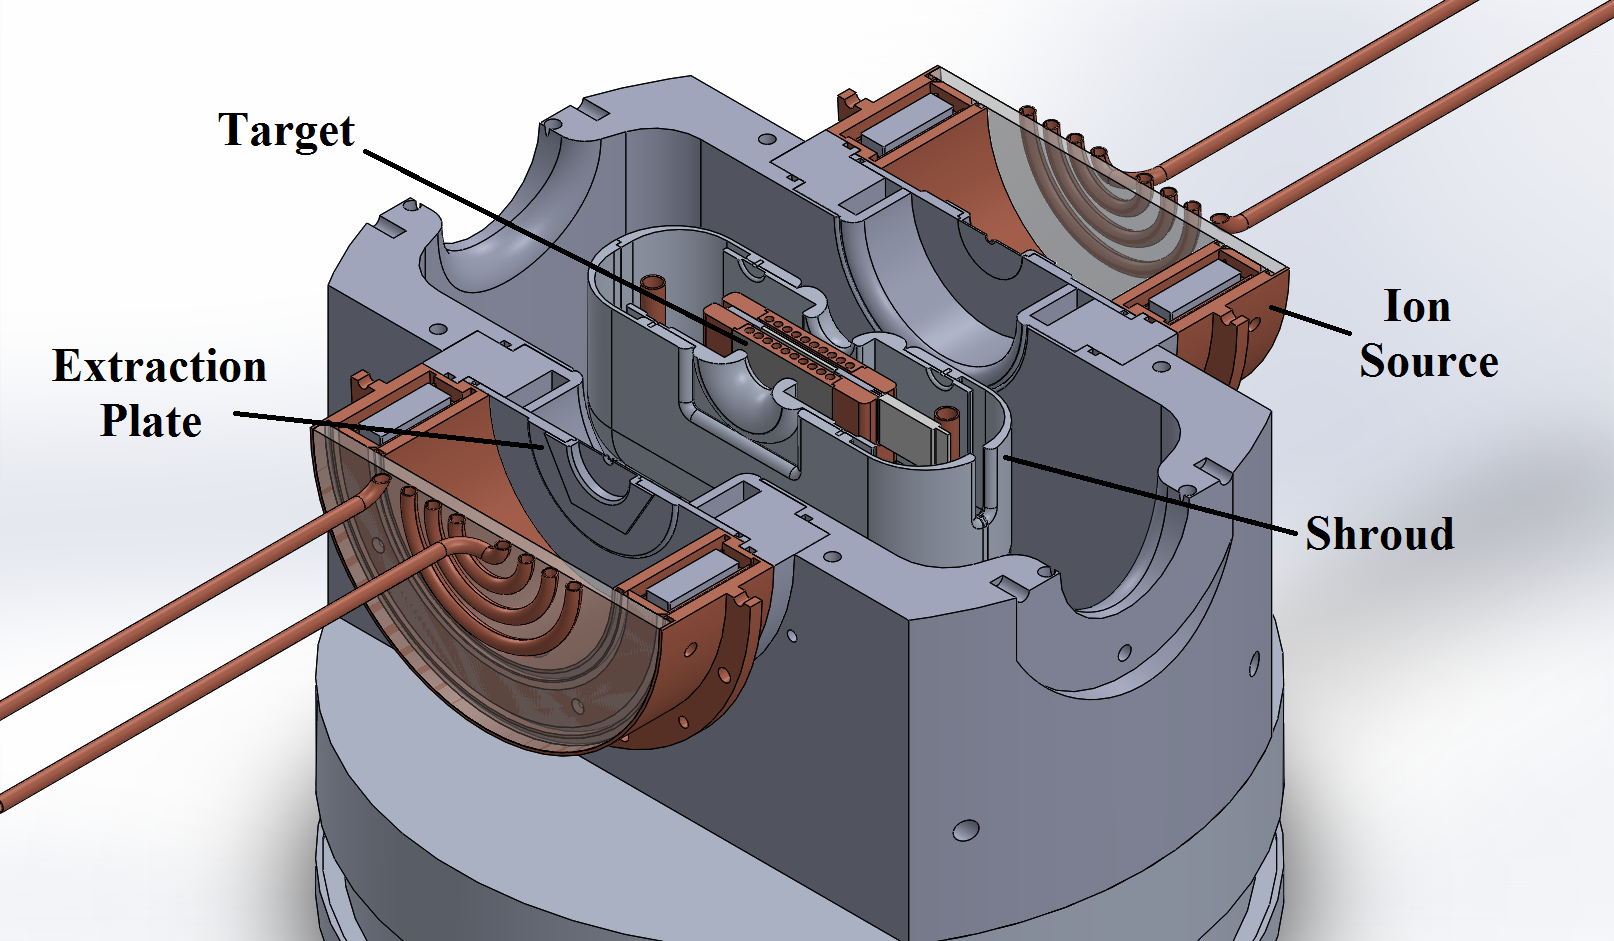
\includegraphics[width=0.5\textwidth]{pics/cutaway}
	\caption{Cross-sectional view of the HFNG exposing the shroud, target, and ion sources.}
	\label{fig:HFNG}
\end{figure}
	
The target, shown in Figure \ref{fig:new_target}, is mostly made of copper due to its excellent thermal conductivity. However, copper does not form hydrides as well as titanium does \cite{CRC}. Therefore, a thin layer (120 microns) of titanium is explosion bonded onto the copper structure. The unique design of this target allows for samples to be placed very close to the neutron emitting spot ($\approx 8 mm$ relative distance), hence maximizing the neutron flux at the sample location. Active cooling with deionized water is needed in order to dissipate the heat load generated by the deuterium beam incident upon the surface of the target. The target is biased at a negative potential (up to -120 kV) in order to extract the positive deuterium ions.

\begin{figure}
	\centering
	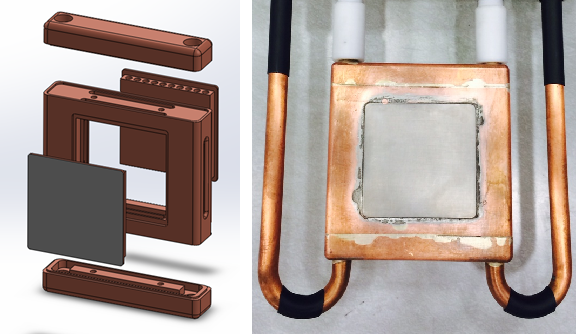
\includegraphics[width=0.5\textwidth]{pics/new_target}
	\caption{Target assembly showing the CAD design of the faceplate and the actual target soldered in place.}
	\label{fig:new_target}
\end{figure}
	
The target is encased in a shroud electrode biased at an even lower potential ($\Delta V=2.4\ kV$) through an arrangement of diodes in order to reverse the direction of the electric field inside this structure. The circuit diagram is shown in Figure \ref{fig:diodes}. Without a shroud, electrons that are sputtered off the titanium target after the deuterium ions impinge on the target would experience a repulsive electrostatic force that would accelerate them back towards the extraction plate causing overheating (or even melting) of surrounding structures, arcing, and a very large flux of bremsstrahlung X-rays. The electric field reversal inside the shroud makes the electrons experience a force back towards the target, which makes them return to it, hence mitigating the issues mentioned above. A detailed discussion of this technique has already been published \cite{electronSup}. 

\begin{figure}
	\centering
	
\includegraphics[width=0.7\textwidth]{pics/diodes3}
	\caption{Circuit schematic of the diode assembly. Note that the voltage differential between the shroud and the target can be varied from 0 to 2.4 kV.}
	\label{fig:diodes}
\end{figure}
	
The vacuum chamber is evacuated by a scroll pump connected in series with a turbo-pump. The scroll pump is oil-free; this is important as the HFNG produces a certain amount of tritium during operation, which readily binds with oil molecules. Furthermore, a scroll pump can be operated continuously without the risk of backstreaming fluids.
	
A polyethylene structure was constructed that can be assembled around the HFNG to thermalize neutrons for different types of experiments. In general, nuclear reactions of the type $(n,\gamma)$ have higher absorption cross-sections at lower energies.

There is also an external beam port aligned with the neutron emitting spot of the HFNG in order to perform experiments outside the vault. Some experiments that have been performed using the external beam line include characterization of gamma detectors in a neutron field, and prompt gamma activation analysis of various materials.   
	
The HFNG uses a residual gas analyzer (RGA) system that allows for continuous/on-line monitoring of the gas composition inside the chamber. It serves as a leak detector as well as a reliable indicator of water vapor, which can cause a variety of problems during operation.
	
	
\section{Neutron Yield, Flux and Energy Distribution}
	
The neutron yield has been experimentally determined in an indirect way. Flux measurements via activation foils were carried out (Section 5) and compared to the simulations presented below. Experimental results agree with those of simulations to about 5\% at the sample holder location. 

Note that a high yield neutron generator does not directly imply a high flux neutron generator. For instance, there are commercially available neutron generators with gas targets with DD neutron yields in the order of $10^{11}\ n/s$. However, the flux at any location around the target is several orders of magnitude lower and impractical for our purposes. Moreover, a neutron generator with a solid target but with a large beam spot compared to the sample also suffers from the same effect. In other words, the yield does not scale linearly with the flux when the beam spot increases. Therefore, the flux is maximized when we operate close to the heat load limit of the target. Hence, a narrow deuterium beam compared to the size of the target is desirable.
	
\subsection{Neutron Yield Analysis}

Some of the accelerated deuterons do not undergo fusion reactions at the energy specified by the voltage differential between the target and the plasma electrode due to two main processes: 1) deuterons slow down as they traverse the target volume before a fusion reaction occurs, and 2) the deuterium beam is not purely monatomic, which also lowers the interaction energy. Both of these processes result in a lower neutron output due to the fact that the DD fusion cross-section decreases with decreasing interaction energy. The slowing down process can be described using data for the energy loss per unit distance (stopping power) of deuterons in titanium \cite{SRIM}. Moreover, the deuterium beam is composed of monatomic, diatomic, and triatomic ion species. The heavier the species, the lower the final energy they achieve for a given target potential. For example, molecular deuterium accelerated to 100 keV will share this energy equally between the two deuterium nuclei i.e. 50 keV each. For RF ion sources, the deuterium is mostly monatomic. However, the exact composition is, for the most part, a function of the RF power. Similar ion sources have been studied \cite{multicusp2} and these reports indicate that at 1200 W (standard for the HFNG), the ratios between the three species are approximately 0.65:0.25:0.10, respectively. Even though RF ion sources produce mostly monatomic deuterium ions, the recombination process is significantly affected by the contact material. Insulators are better at hindering recombination, while conductors such as copper have much higher recombination coefficients.  

The neutron yield can be approximated based on an analytical approach outlined in \cite{CRC} together with empirical data for the stopping power ($dE/dx$) of deuterons in titanium, the cross-section for the neutron-producing reaction in Equation \ref{eq:reactionDD}, the fraction of different deuterium species in the ion source, and the deuterium-to-titanium ratio in the self-loaded target, which was taken to be one-to-one for a conservative estimate. Equation \ref{eq:yield} was used to calculate the neutron yield as a function of deuteron energy, where $\phi_d$ is the deuteron flux ($cm^{-2}s^{-1}$) incident on the target, $n_d$ is the number density of deuterons in the target ($cm^{-3}$) when saturated, $\sigma(E_d)$ is the cross section for the DD neutron-producing reaction, and $dE/dx(E_d)$ is the energy loss per unit distance in titanium. Note that the lower limit of integration is taken to be zero since the Q-value of the reaction is positive. The yield calculated with this equation is an input for the MCNP \cite{MCNP} model, which calculates the neutron flux per source particle. This approach agrees with experiments relatively well, as discussed in the last section. 

\begin{equation} \label{eq:yield}
Y(E_d)=\phi_d n_d \int_{0}^{E_{max}} \frac{\sigma(E_d)}{dE/dx(E_d)}dE_d
\end{equation}

	
\subsection{Neutron Flux and Energy Distribution}

The kinematics of the interaction between deuterons results in a variation of neutron energy as a function of angle in the lab frame. From energy and momentum conservation, the energy of the emitted neutron varies as shown in Figure \ref{fig:energy_dist}. Note that the variation can be quite significant. For instance, at zero deuteron incident kinetic energy, the energy of the emitted neutron is 2.45 MeV, while at 100 keV, the maximum is close to 2.8 MeV. The apparent violation of the conservation of energy principle is accounted for by the redistribution of the total available energy (Q-value plus incident deuteron energy) between the He-3 nucleus and the neutron. 

\begin{figure}
	\centering
	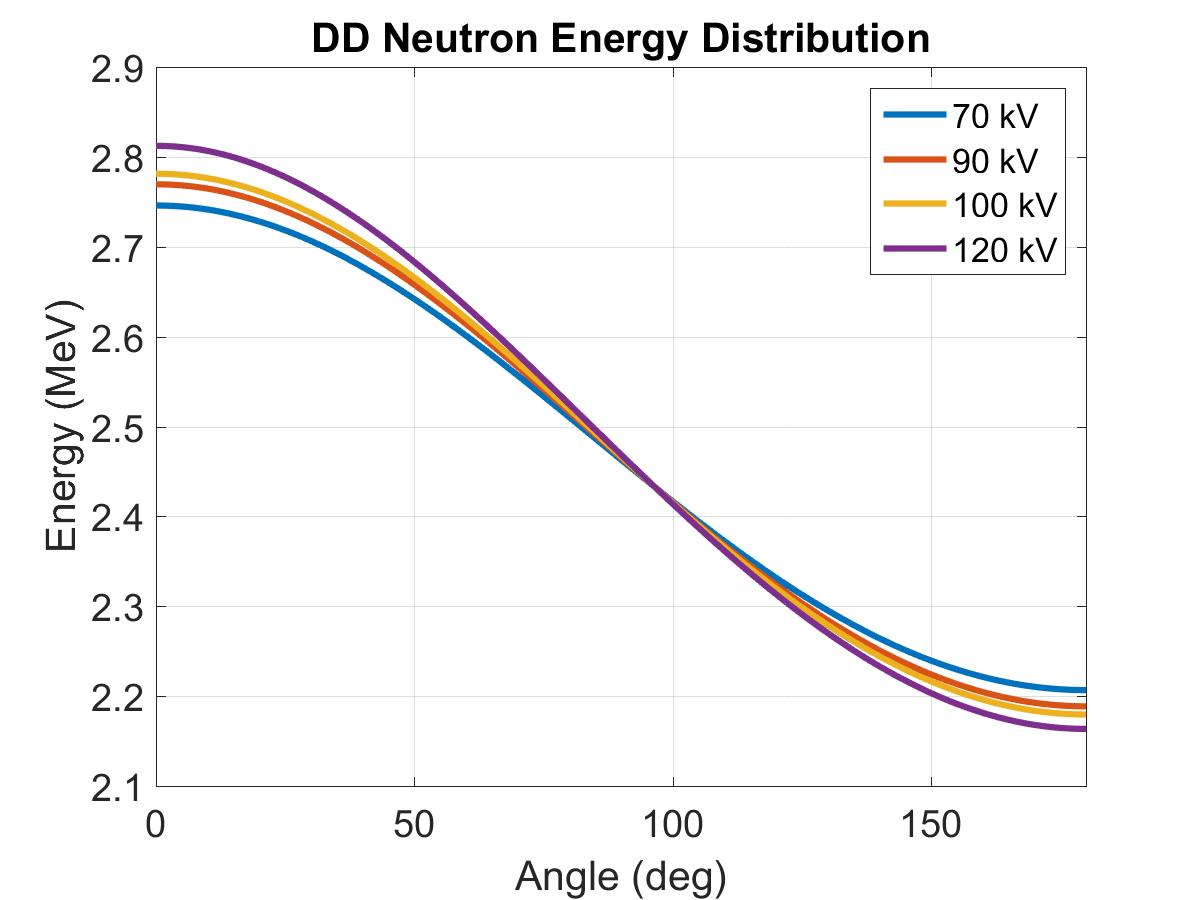
\includegraphics[width=0.7\textwidth]{pics/energy_dist}
	\caption{Neutron energy in the lab system as a function of angle.}
	\label{fig:energy_dist}
\end{figure}

The energy spectrum changes slightly as the neutron travels through the target. Therefore, different empirical correlations were found for thin and thick targets \cite{CRC}. The angular distribution is well-fitted with an expansion in Legendre polynomials, as shown in Equation \ref{eqn:energDist}. Note that this equation is valid for DD and DT reactions below $500\ keV$ for both, thin and thick targets. 

\begin{equation}
E_n(E_d,\theta)=E_0+\sum_{i=1}^{n}E_i cos^i \theta
\label{eqn:energDist}
\end{equation}

The coefficients $E_i$ were determined for a few energy values only \cite{CRC}. Therefore, they were interpolated in this code using a cubic spline for any desired energy.

Furthermore, the neutron yield is also dependent on the emitted angle, and DD neutrons exhibit a larger anisotropy than DT neutrons. The highest yield in this kind of neutron generators is along the deuteron beam direction ($0^\circ$). The relative yield, defined as the total yield normalized to that at $90^{\circ}$, can be described by Equation~\ref{eqn:angDist}. This equation comes from a best fit model of the available data \cite{CRC}.

\begin{equation}
\frac{Y(\theta)}{Y(90^{\circ})}=A_0+\sum_{i=1}^{n}A_i cos^i \theta
\label{eqn:angDist}
\end{equation}

The coefficients $A_i$ were interpolated using a cubic spline for any desired voltage value. Figure~\ref{fig:yield} shows the relative yield distribution in the lab frame for various voltages.

\begin{figure}[H]
	\begin{center}
		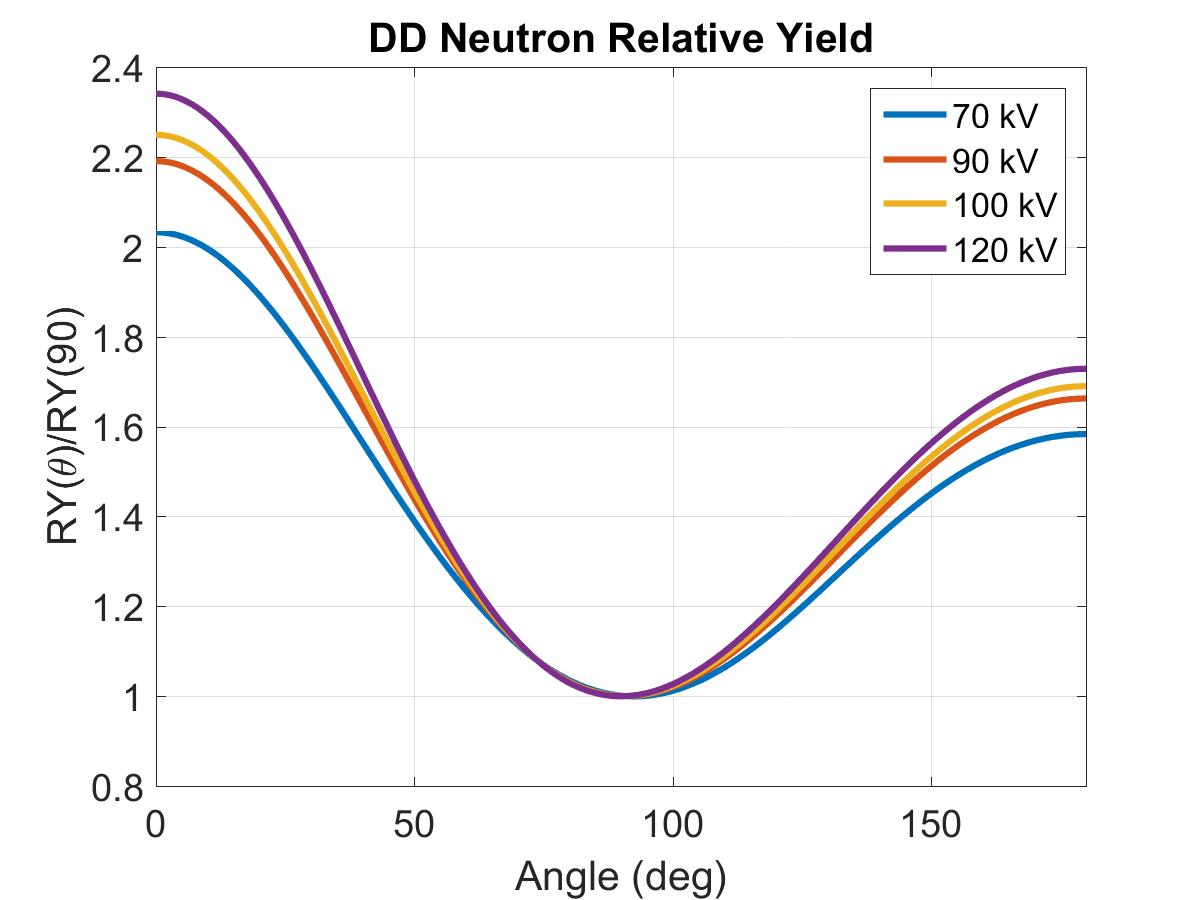
\includegraphics[width=0.7\textwidth]{pics/rel_yield} 
		\caption{Relative neutron yield for different accelerating voltages (DD reactions).}
		\label{fig:yield}
	\end{center}
\end{figure}

We developed an MCNP model of the generator and surrounding structures. The neutron source is modeled according to experimental data obtained from \cite{Cross_sections}. The main purpose of such a model is to obtain the flux and energy distributions at different irradiation locations. The titanium target is considered to be ``thick'' in the sense that all accelerated deuterons either interact or stop within the target; deuterons penetrate the target a maximum of just under 1 micron at 120 kV, while the titanium layer is several hundred micrometers thick. The types of neutron sources considered in the MCNP model were point-like, disk, and Gaussian shaped, with the latter being the more accurate representation of the actual source (single-hole extraction). The code developed allows for different input parameters to be modified according to the experiment being performed. Such parameters include the acceleration voltage, the deuterium ion current, the atomic deuterium ion fraction in the plasma, the beam diameter, and the Gaussian profile of the beam. These results are shown in Figure \ref{fig:source_definitions}. Note that there is no significant difference among the three different source definitions for this specific case. However, if the irradiation location or the size of the samples change, it is important to re-check that these definitions agree.   

\begin{figure}
	\centering
	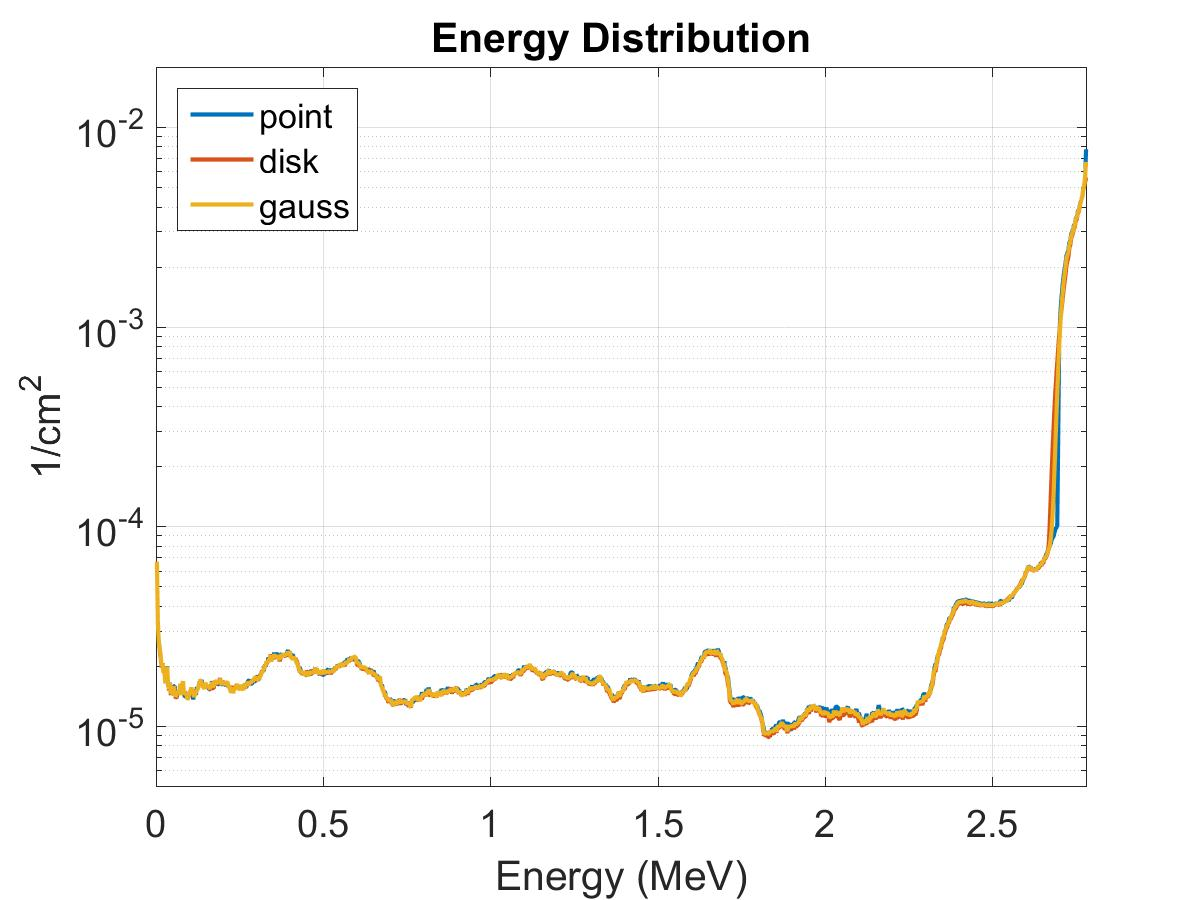
\includegraphics[width=0.7\textwidth]{pics/comp_sources_log}
	\caption{MCNP simulations for different source definitions in terms of energy distribution at the center of the sample holder location. Units on the y-axis are normalized per source neutron.}
	\label{fig:source_definitions}
\end{figure}

In order to take advantage of the variation of neutron energy as a function of angle, a L-shaped sample holder was designed and machined so that samples can be located in such a way as to span neutron energies between 2.4 - 2.8 MeV at 100 kV extraction voltage, as shown in Figure \ref{fig:L_holder}. This arrangement is particularly interesting for cross section measurements at different neutron energies. It has been used for $^{35}Cl(n,p)$ and $^{35}Cl(n,\alpha)$ reaction cross section measurements. The size of the energy window depends on the size of the sample, and MCNP simulations should be performed in order to quantify this energy spread. The sample slot located at $98^{\circ}$ allows for a ``clean'' neutron beam, which means that there is virtually no structural material in between the sample and the neutron emitting spot. This arrangement allows for a more narrow energy distribution, but at the expense of a reduced neutron flux due to the $1/r^2$ dependence and the kinematics of the reaction, as shown in Figure \ref{fig:yield}. 

\begin{figure}
	\centering
	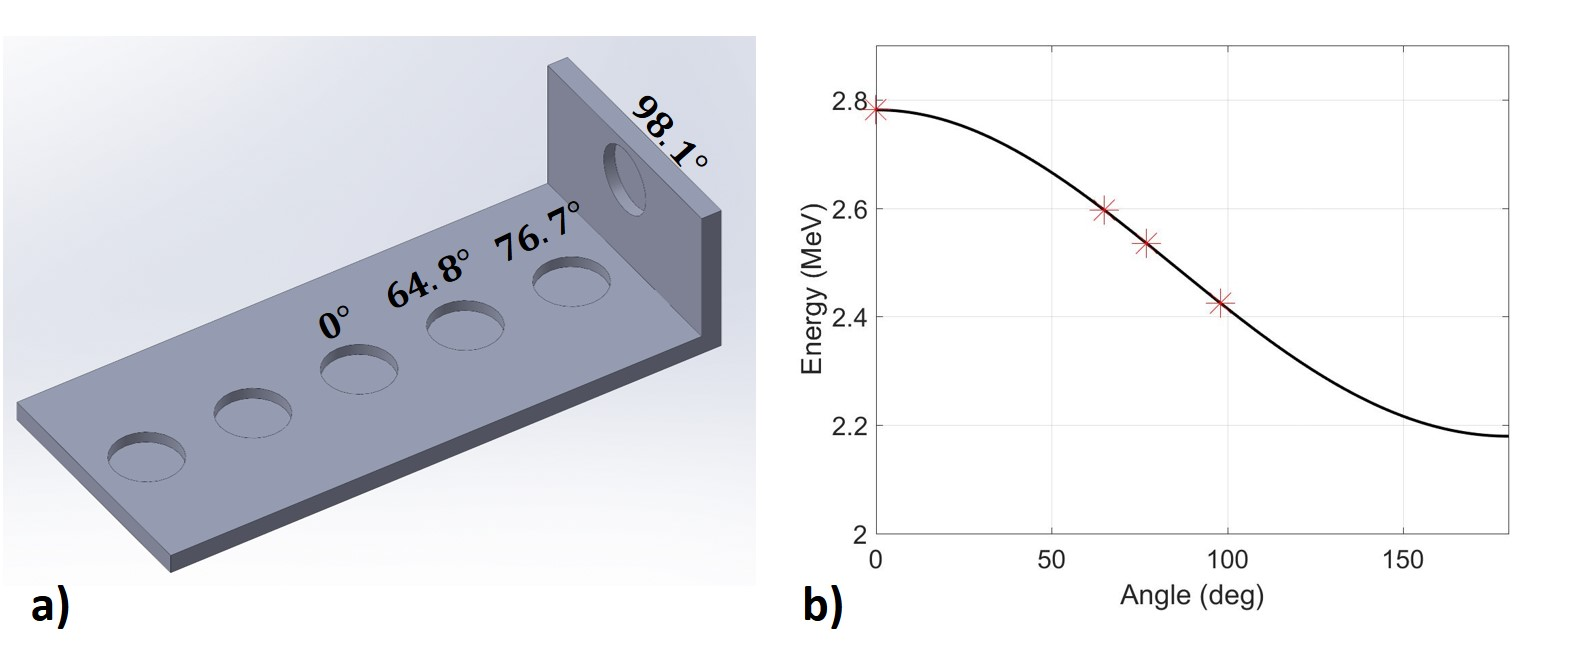
\includegraphics[width=1\textwidth]{pics/L_holder_ang2}
	\caption{Sample holder that allows for irradiation of samples at different neutron energies. The values shown correspond to a 100 kV extraction voltage.}
	\label{fig:L_holder}
\end{figure}
	
\section{Ion Beam Extraction Analysis}

The deuterium beam is extracted from the plasma electrode of the ion source through either one or multiple apertures. The configuration and design of such an extraction mechanism largely determines the beam profile. Precise knowledge and control of the ion optics is necessary in order to 1) achieve a uniform beam profile on the surface of the target and 2) prevent the localized temperature to reach $\sim 200^{\circ}\ C$ \cite{AANG}. The first requirement ensures that the resulting neutron flux is also uniform over the sample to be irradiated, which is essential for several experiments such as the irradiation of geological samples \cite{geochron}. The second requirement has to do with the fact that deuterium degases from titanium around this temperature, which results in a lower neutron output. Moreover, if the heat load surpasses a certain value determined by the specific target configuration, the target can be eroded and destroyed. 

The optimum beam spot size varies according to the application of the neutron generator. For example, a very small spot size is needed for fast neutron imaging because it enhances the sharpness of the image \cite{adams}. However, this requirement limits the beam current the target can handle, which in turn, limits the neutron yield at a given acceleration voltage. The HFNG allows for a variety of (exchangeable) extraction plate designs that result in different beam profiles depending on the application. Extensive analysis and modeling was performed for a single extraction aperture of 0.262 cm in diameter and a multiple-hole extraction plate.

A flat plasma meniscus at extraction is desired in order to achieve a uniform beam profile \cite{CoryThesis}. However, precise modeling of the plasma meniscus is complicated due to all the variables involved and the imperfect fidelity of plasma physics simulations (specially near plasma boundaries). Moreover, slight changes in electron temperature and ion density in the plasma affect the shape of the plasma meniscus, as determined by Bohm's Equation \cite{plasma}. Nevertheless, as the diameter of the extraction aperture decreases, the effects of the plasma meniscus on the resulting beam profile are greatly reduced, and at very small ($\sim 1\ mm$) apertures, the extracted beam is barely affected by focusing or defocusing effects due to the shape of the plasma meniscus.   

The finite-element software package Comsol Multiphysics was used in order to simulate the ion beam trajectory for a single extraction aperture nozzle of 0.262 cm diameter and a 19-hole extraction electrode (each 1 mm id diameter), as shown in Figure \ref{fig:single_vs_mult}. The geometry of the setup is accurately represented as it is imported from a CAD program. The assumptions built into the simulations are as follows.

1) Ions are extracted from a flat plasma meniscus, which is a reasonably good assumption because of the small size of the extraction aperture and when operated near the Child-Langmuir limit.

2) All ions are born with the same speed and with a perpendicular velocity to the surface of the plasma. Even though the energy of the ions in the plasma follows the Maxwell-Boltzmann distribution, this assumption encompasses the overall behavior of the beam as it travels to the target. 

Figure \ref{fig:beam_spread} shows the electric potential and the simulated particle trajectories at a target bias and beam current of 100 kV and 1.4 mA, respectively. Note in Figure \ref{subfig:beam_spread} that the equipotential lines near extraction result in a slightly focusing field. This is due to the geometry of our setup that required the ion source to be recessed back a certain distance in order to achieve the desired current density, reduce the maximum electric field in that region, and allow for the beam to spread so the heat flux on the surface becomes acceptable.

\begin{figure}
	\centering
	\subfloat[\label{subfig:beam_spread}]{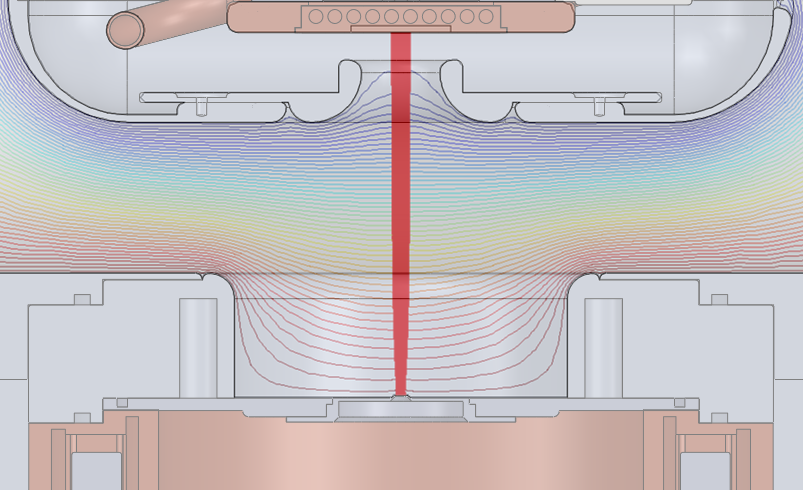
\includegraphics[width=0.55\textwidth]{pics/beam}}
	\hfill
	\subfloat[\label{subfig:beam_in_shroud}]{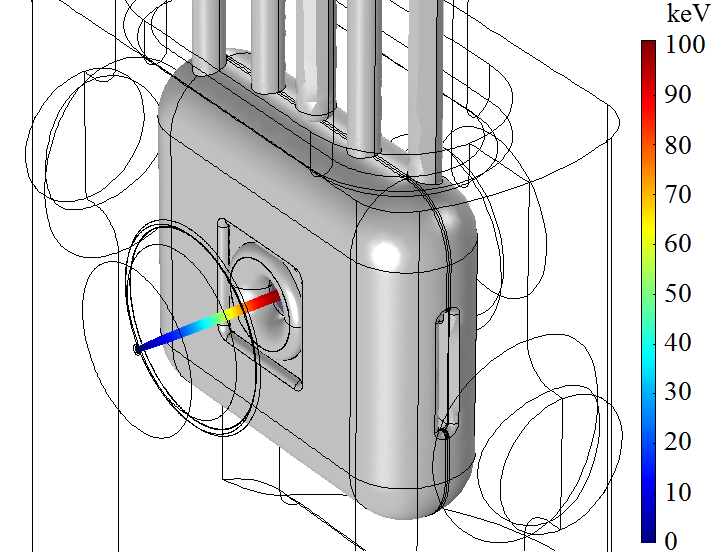
\includegraphics[width=0.445\textwidth]{pics/beam_shroud}}
	\caption{Comsol simulation of electric field and deuteron beam trajectory at 100 kV and 1.4 mA.}
	\label{fig:beam_spread}
\end{figure}

The resulting beam spot size and heat deposition on the target are shown in Figure \ref{fig:beam_spot2}. Note that the beam profile in a) is not uniform across the target, and there is localized heating (and neutron production) near the edges. Therefore, a convex-shaped extraction nozzle was designed, whose purpose is to counteract the focusing electric field experienced near the aperture. The nozzle design is shown in Figure \ref{fig:beam_spot2} b) and c). Note the defocusing effect of the nozzle due to the fact that the equipotential lines are slightly convex downstream of the beam path. The beam spot is not only more uniform, but it is also spread throughout a larger area, which reduces the heat load on the target.

\begin{figure}
	\centering
	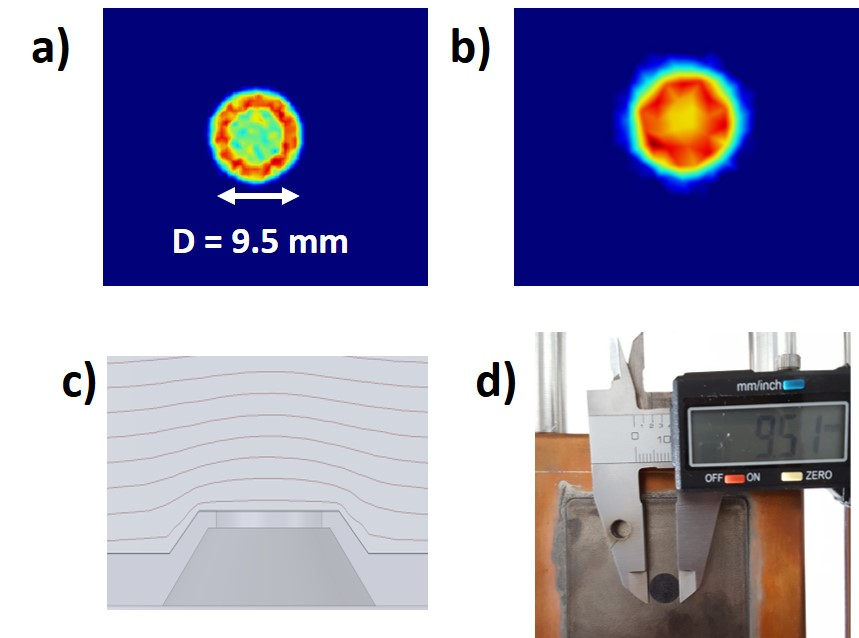
\includegraphics[width=0.7\textwidth]{pics/beam_spot2}
	\caption{Beam spreading by modification of the extraction plate: a) flat extraction, b) and c) convex extraction, d) burn mark on target.}
	\label{fig:beam_spot2}
\end{figure}

Experimental results show a high degree of consistency with simulations based on the beam spot size (diffuse burn mark measured to be around 10 mm), and the resulting neutron flux distribution, as detailed in Chapter 5. 


\subsection{Multiple-Hole Extraction System}

The uniformity of the beam spot and further spread of impingement area can be achieved by different means. For instance, an Einzel lens configuration, i.e. one or more extraction plates located downstream of the beam and biased at different potentials can give further control of the beam envelope. One of the downsides of such an arrangement is the higher degree of complexity added to the design, which stems from biasing, insulating, and properly installing these plates inside the vacuum chamber. Another option is the use of multiple apertures in the plasma electrode. Figure \ref{fig:CAD_extraction} shows an optimized design of a 19-hole extraction plate arranged in a hexagonal pattern, which was chosen in order to optimize the packing fraction and the uniformity of the beam.

\begin{figure}
	\centering
	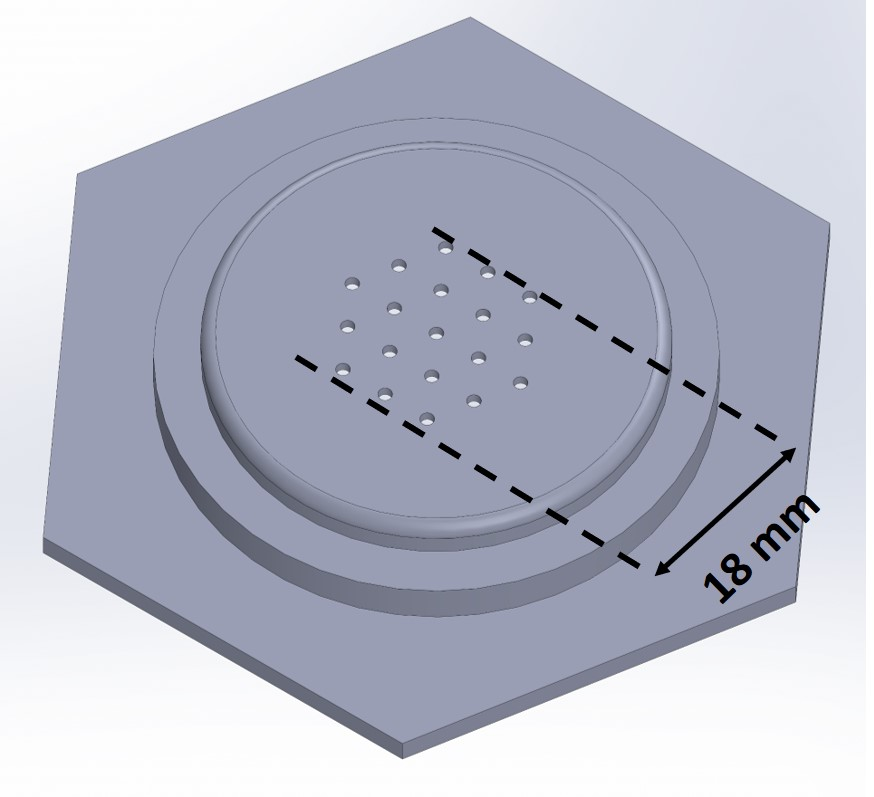
\includegraphics[width=0.5\textwidth]{pics/CAD_plate2}
	\caption{CAD drawing of an optimized 19-hole extraction plate.}
	\label{fig:CAD_extraction}
\end{figure}

In order to approximate the maximum beam current that can be extracted from each individual hole, the Child Langmuir law was employed, which sets a limit for the extractable current through an aperture assuming the system is space charge limited (enough ions are available in the ion source). This treatment was derived only for beam extraction between parallel plates, but serves as a good approximation for our purposes. Figure \ref{fig:child_lang} shows the maximum theoretical beam current that can be extracted as a function of the aperture diameter for the HFNG geometry at 100 kV. Because it is in our interest to keep the diameter of the apertures small, we chose a diameter of $1\ mm$, through which it is possible to draw a current of $\approx 0.196\ mA$. Therefore, for the 19-hole plate arrangement, it is theoretically possible to draw up to $3.7\ mA$, or a total of $7.4\ mA$ if both ion sources are used. This current value is an approximation, but it serves as a conservative input parameter for the ion beam simulations. In fact, the observed current limit was 3.5 mA, confirming the validity of this approximation.

 \begin{figure}
 	\centering
 	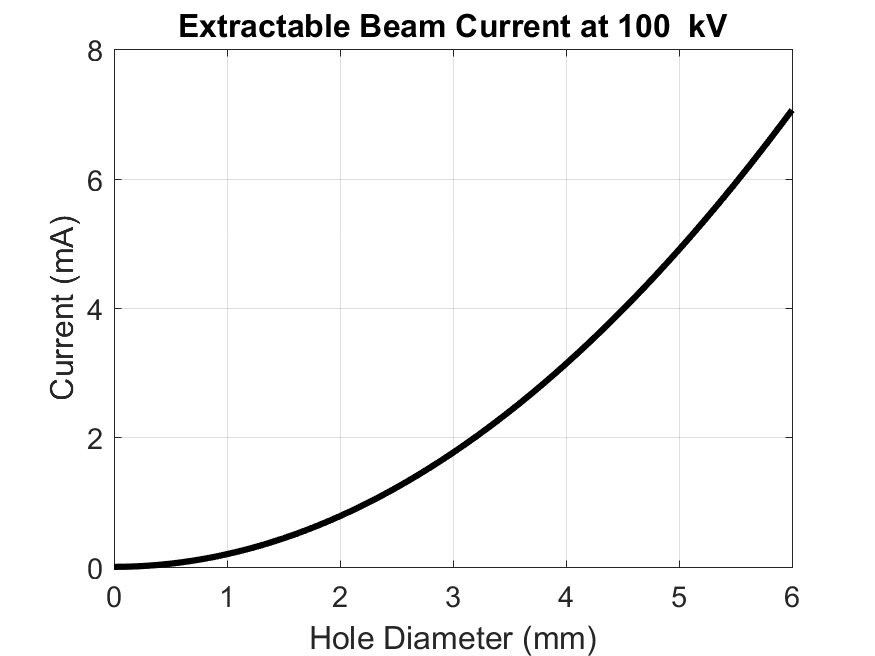
\includegraphics[width=0.7\textwidth]{pics/childLang}
 	\caption{Maximum extractable current according to Child Langmuir law for the HFNG geometry at 100 kV.}
 	\label{fig:child_lang}
 \end{figure} 

Simulations show a more uniform beam profile near the center and a larger impingement area, which translates into a lower heat flux than that of a single hole even at higher current values. Beam current can be further increased by adding more holes or by increasing the size of the holes. The increase in current can be limited by the maximum number of holes that can be drilled on the plate or by the increase in chamber pressure due to a larger open area between the ion source and the rest of the vacuum chamber. The latter could make the gas pressure too high for optimum operation. 

The geometry of the HFNG is such that there exists a focusing electric field at extraction, as shown in Figure \ref{fig:beam_spread}. Therefore, off-centered beamlets experience a focusing force, which depends on their location with respect to the center. For instance, beamlets further away from the center experience a stronger focusing force because the equipotential lines are more concave in that region. Therefore, multiple-extraction hole systems produce a convergent beam envelope. In contrast, a single hole in the center produces a divergent beam envelope, as shown in Figure \ref{fig:single_vs_mult}. The reason for this spread is somewhat due to space charge. However, the main reason is the initial focusing provided by the extraction hole itself, which causes deuterons to cross over and then diverge. This phenomenon is depicted in Figure \ref{fig:cross_over}. Essentially, each extracting aperture acts as a non-linear electrostatic lens with spherical aberration (not focused to a point) \cite{Plasma}. 

\begin{figure}
	\centering
	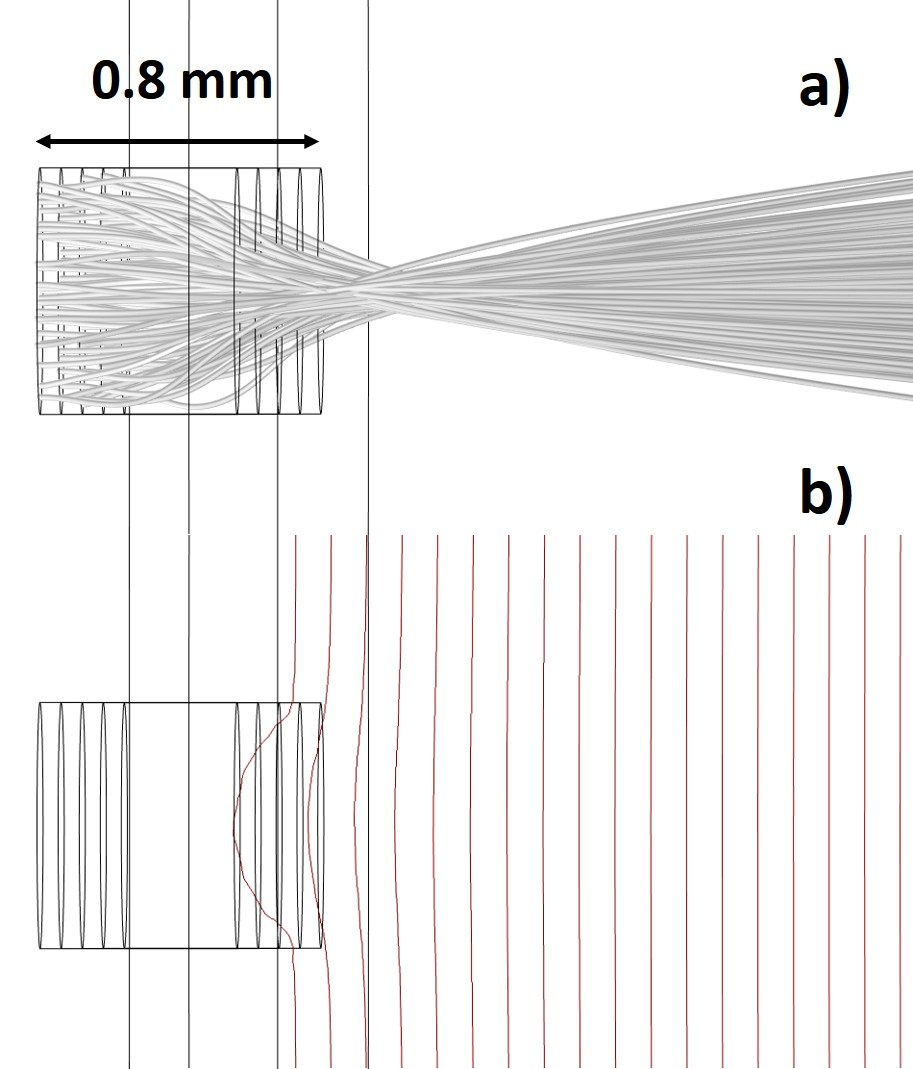
\includegraphics[height=0.6\textwidth]{pics/cross_over_comp}
	\caption{Simulation of deuteron trajectories near extraction. Note the convergent field (b) that provides the initial focusing force that is ultimately responsible for the spreading of the beam.}
	\label{fig:cross_over}
\end{figure}

\begin{figure}
	\centering
	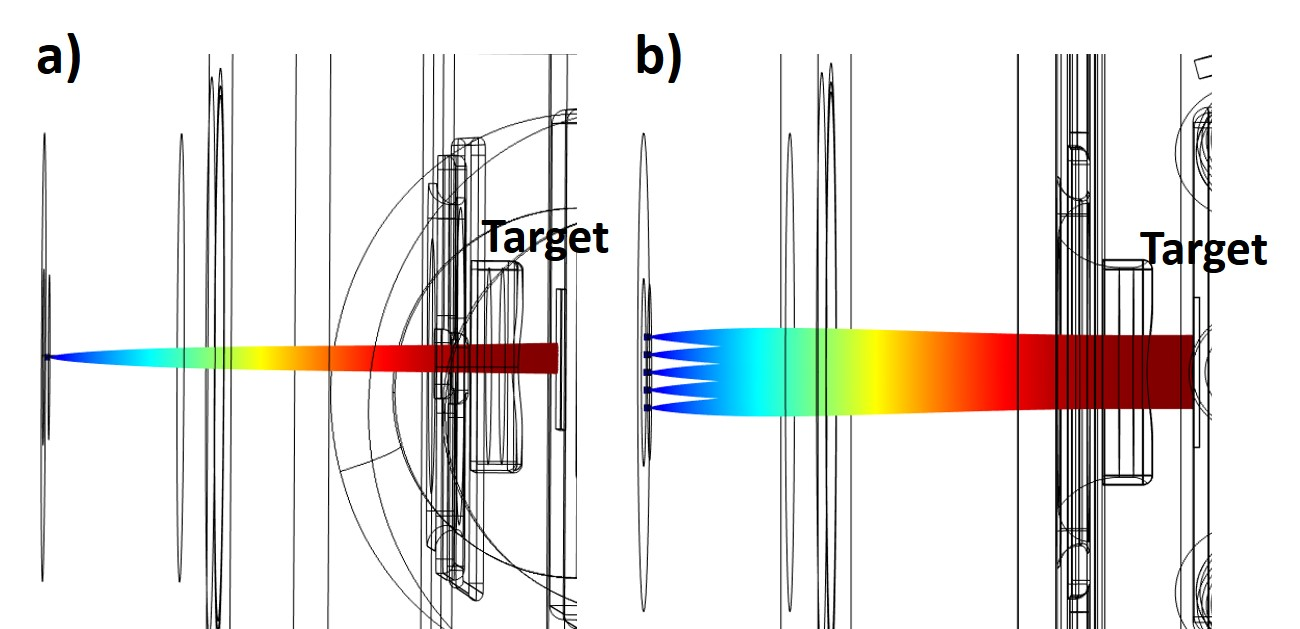
\includegraphics[height=0.5\textwidth]{pics/single_vs_mult2}
	\caption{The beam envelope for a single beam located at the center is divergent while that of multiple holes is convergent.}
	\label{fig:single_vs_mult}
\end{figure}

If there were no spacer, the beamlets would not experience a focusing force and the beam envelope would be divergent, as shown in Figure \ref{fig:spacer_vs_noSpacer}. However, at such a close distance ($\approx 7\ cm$ from the target), the individual beamlets would not spread enough and the heat deposition per beamlet would be unacceptable.  

\begin{figure}
	\centering
	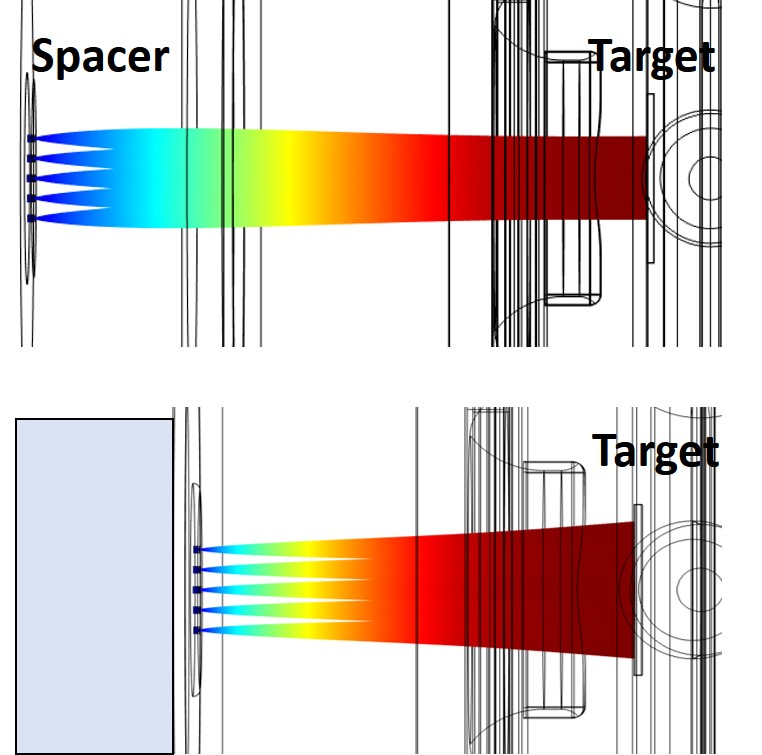
\includegraphics[width=0.5\textwidth]{pics/spacer_vs_noSpacer2}
	\caption{Beam envelope with spacer (top), and without spacer (bottom), showing the effect of the spacer, which gives an additional standoff of 7 cm; the spacer also introduces a focusing field.}
	\label{fig:spacer_vs_noSpacer}
\end{figure}
 
Simulations were performed in order to optimize the hole pattern distribution. The design curve shown in Figure \ref{fig:designC} shows the beamlet center at the target as a function of the beamlet location at the extraction plate. The dashed line shows the hypothetical case in which there is no focusing field and the beamlets are perfectly horizontal. 

\begin{figure}
	\centering
	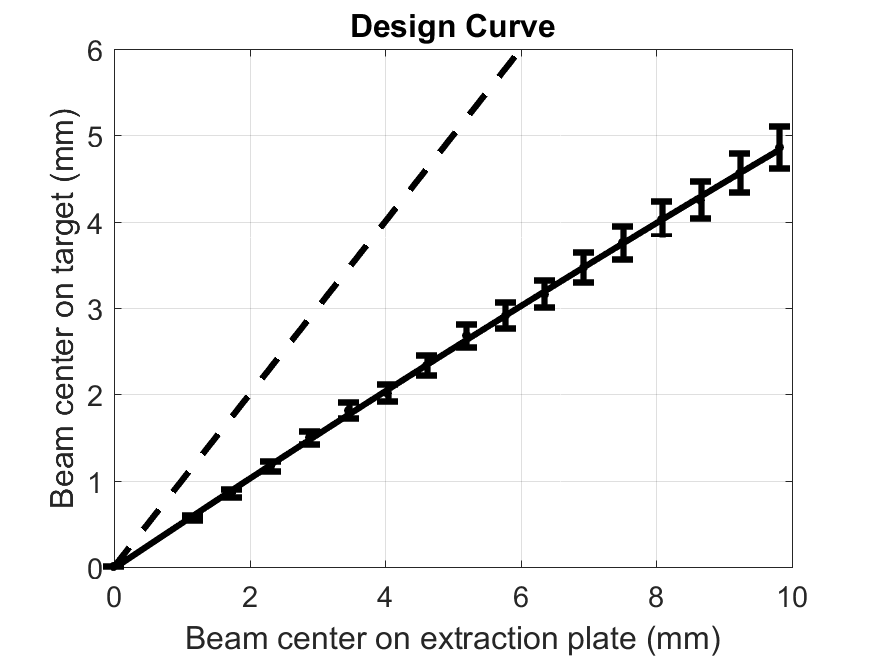
\includegraphics[height=0.5\textwidth]{pics/designC}
	\caption{Design curve used to estimate the center of the individual deuterium beamlets on the target. The dashed curve is for the case with no spacer (linear) and the solid curve for the current configuration.}
	\label{fig:designC}
\end{figure}

The optimization process focused on two parameters: reduction of heat flux on the target surface, and uniformity of the heat flux distribution, which translates into a more uniform (flat) neutron flux distribution at the sample location.

\begin{figure}
	\centering
	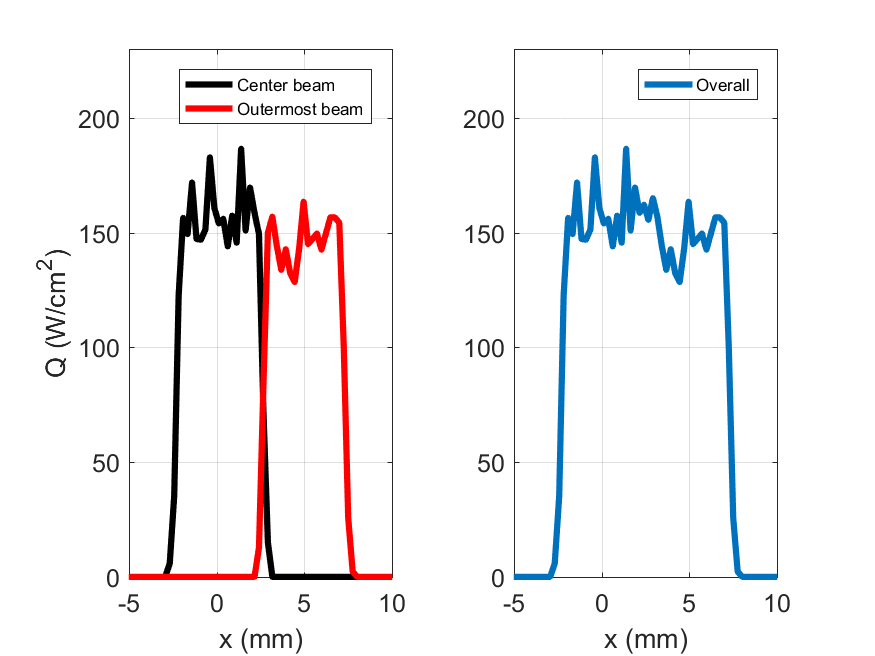
\includegraphics[height=0.5\textwidth]{pics/twoBeams}
	\caption{Comsol simulation results showing the center and outermost beamlets. The latter was placed so as to achieve a flat profile.}
	\label{fig:two_beams}
\end{figure}

Figure \ref{fig:two_beams} shows the 2D beam profiles of the center beamlet and the outermost beamlet. The latter was placed 9.8 mm from the center in order to achieve a flat beam profile on the target. The intermediate hole was placed in such a way that its corresponding beamlet would hit the target exactly midway between the other two. This location was calculated (from the design curve) to be 5.1 mm from the center. The resulting heat flux distribution is shown Figure \ref{fig:heat maps} (right). Note that evenly spaced extraction apertures result in a non-uniform distribution due to the uneven focusing effect explained previously. A design leading to an unacceptable heat profile is shown in Figure \ref{fig:heat maps} (left). 

\begin{figure}
	\centering
	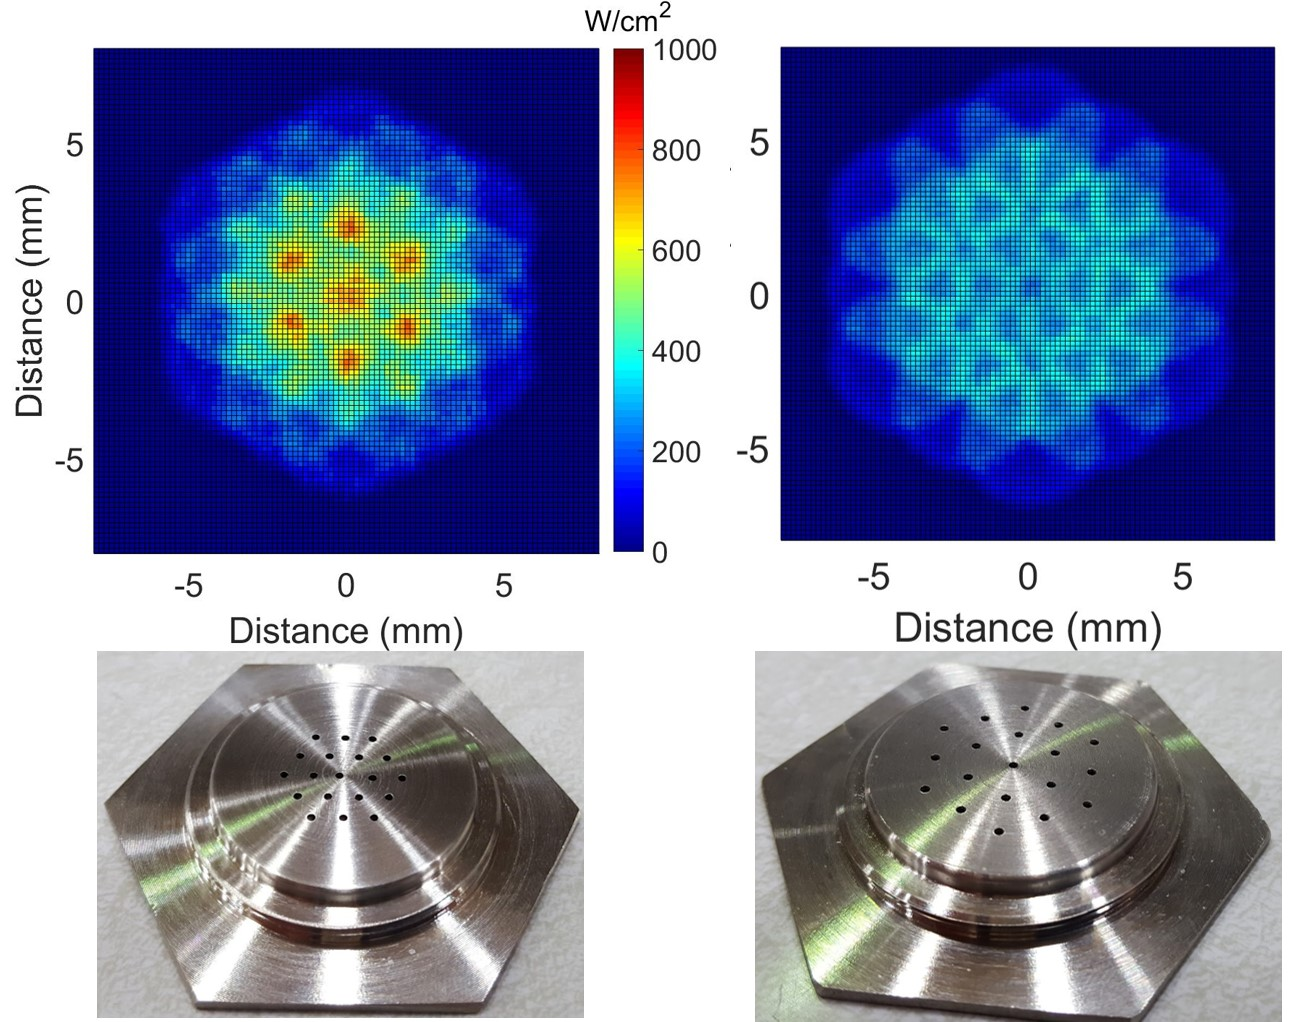
\includegraphics[height=0.6\textwidth]{pics/comparisonHeatMaps_plates2}
	\caption{Power density on the target for a non-optimized design (left) and a design optimized according to the design curve shown in Figure \ref{fig:designC}. }
	\label{fig:heat maps}
\end{figure}

Note that even though the spacing between the holes is larger on the optimized extraction plate design ($d \approx 2 \ cm$), the resulting beam profile on the target is similar in size as the non-optimized design ($d\approx 1.1 \ cm$), but with a higher degree of uniformity and reduced heat flux. Experimental tests validate these simulations, as shown in the experimental validation section.

\subsection{Heat Transfer Analysis}

The heat flux distribution on the target surface was modeled in Comsol using the heat transfer in solids module coupled with the turbulent flow module. Further details about the heat transfer analysis on the target can be found in \cite{CoryThesis}. Figure \ref{fig:temp_comsol} shows the temperature distribution on the surface of the target for three different beam profiles: single hole, non-optimized multiple-hole, and optimized multiple-hole extraction plate. Note that the three of them show maximum temperature values below the degassing temperature of hydrogen in titanium ($\approx 230\ ^{\circ}C)$. However, the simulations do not account for the inter-metallic phases between the copper and the titanium, or the bonding process itself. Experimentally, it was found that the neutron yield is lower in the case of diffusion bonding compared to the explosion bonded material. This might indicate that the latter has better heat transfer properties. Moreover, variations in the titanium thickness an purity of the metal can also affect the neutron yield. The thinner the titanium layer, the better the heat transfer properties of the target. The disadvantage of having a very thin titanium layer is that the target has a shorter lifetime due to ion sputtering.


\begin{figure}
	\centering
	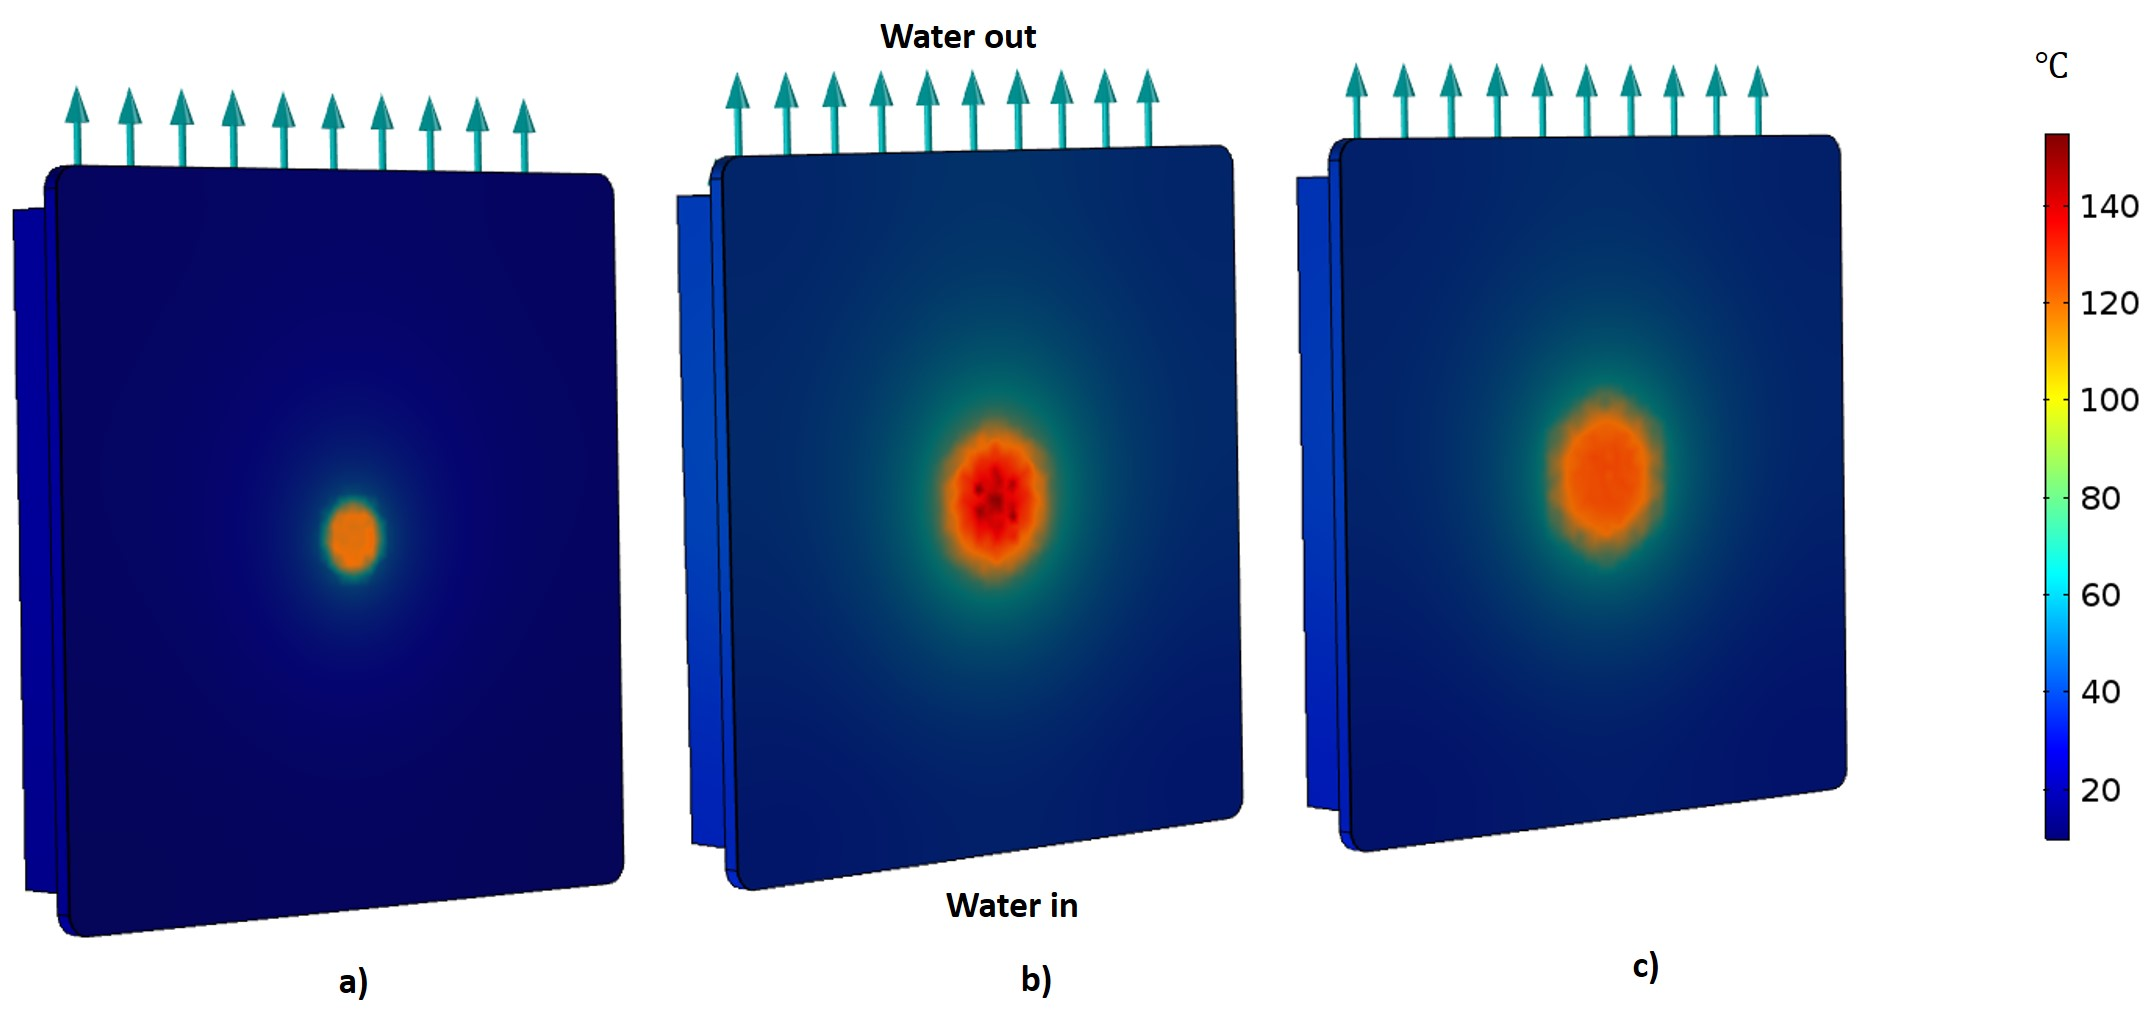
\includegraphics[height=0.5\textwidth]{pics/temp_profiles2}
	\caption{Temperature maps on the target for different extraction plates a) single-hole b) multiple-hole, non-optimized, c) Multiple-hole optimized. Maximum temperature values are $104^{\circ}C$,  $155^{\circ}C$,  $114^{\circ}C$, respectively}
	\label{fig:temp_comsol}
\end{figure}

\begin{figure}
	\centering
	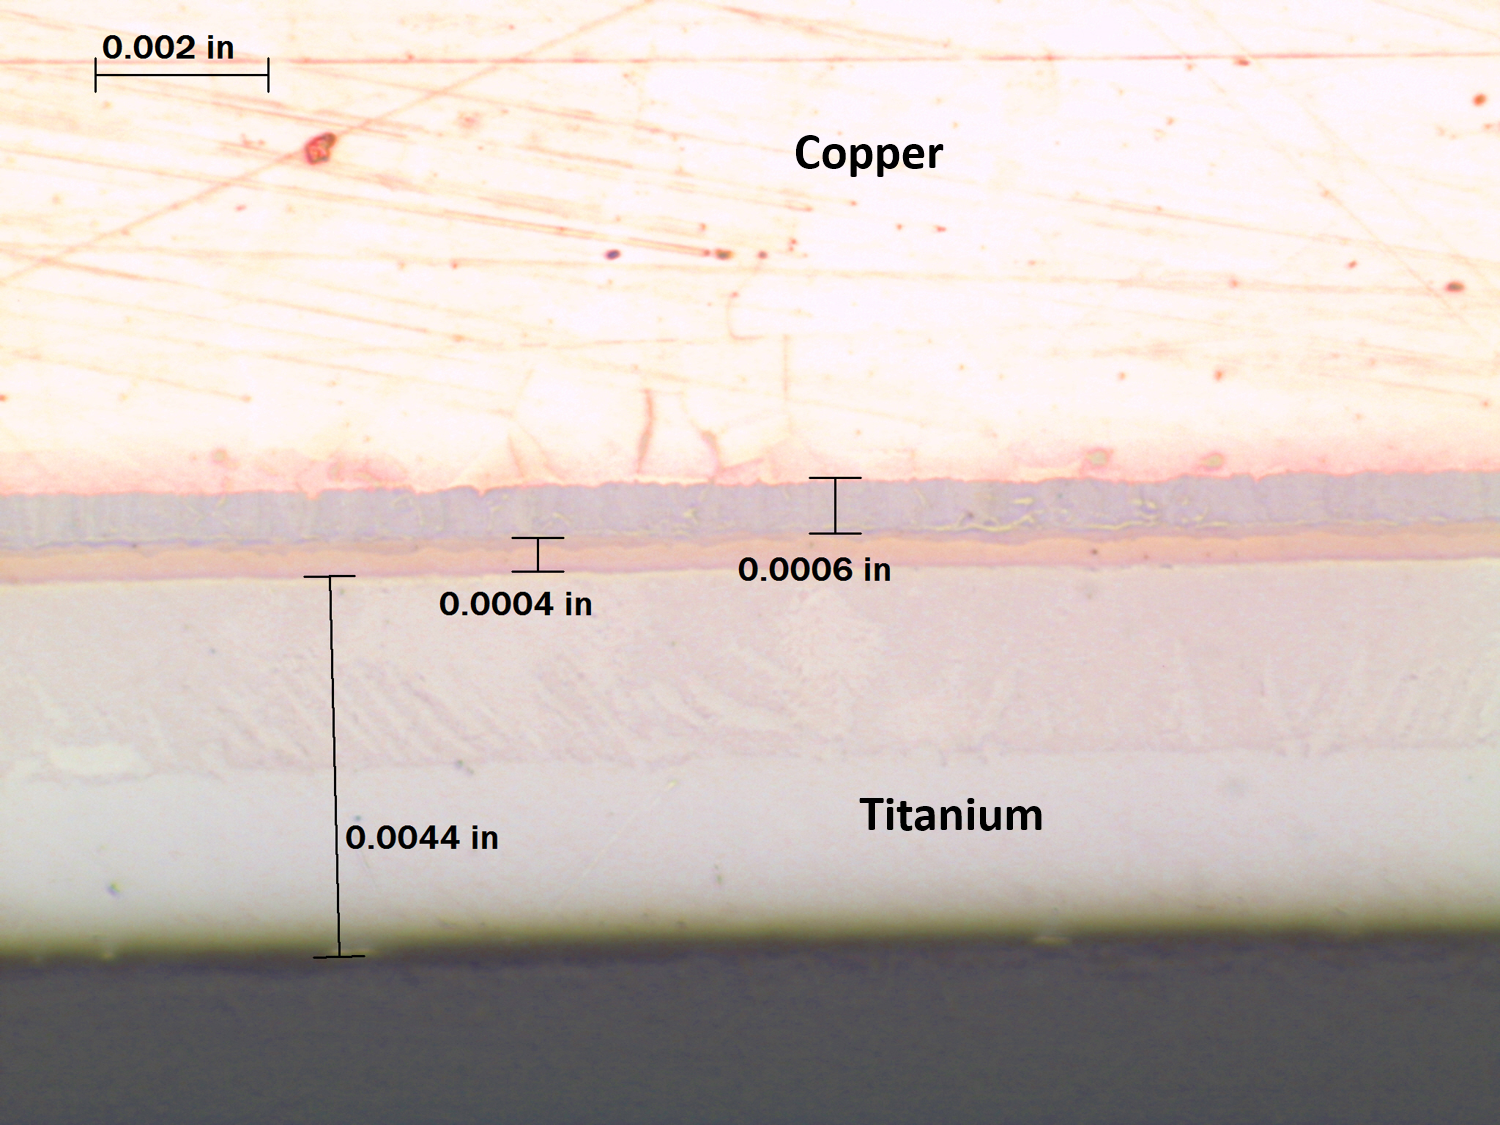
\includegraphics[height=0.5\textwidth]{pics/TiCu2}
	\caption{Metallographic test on the HFNG target showing the intermetallic phases between copper and titanium.}
	\label{fig:TiCu}
\end{figure}

Figure \ref{fig:TiCu} shows a metallographic test of the diffusion bonded target. Note that there is a region of about 25 $\mu m$ in the copper-titanium interface with two visible phases (CuTi intermetallics), which is difficult to include in the simulations and their effect on the heat transfer is unknown. However, the titanium thickness in the simulated model can be increased by that amount in order to remain conservative. Experimentally, it was determined that there is some overheating of the target in the case of the non-optimized extraction plate. This was evidenced by the initial increase in neutron dose rate rapidly followed by a decrease rate. The neutron yield in this case was similar to that of the single-hole extraction plate. However, the optimized geometry allows for an increase in neutron yield by a factor of $\approx 2.5$, which is expected from Equation \ref{eq:yield}.      
 
	
\section{Experimental Validation of the Neutron Flux and Deuteron Beam Profile}	

The neutron flux was experimentally determined by neutron activation analysis of nine natural indium foils arranged in a $3\times3$ array at the sample holder location shown in Figure \ref{fig:flux_map}. Indium is a soft metal that can be easily cut or machined to the desired size and shape. The foils were cut in the form of thin disks of about 0.9 cm in diameter. The isotope In-115 has a long lived ($t_{1/2}=4.486\ h$) isomer that decays by the emission of a 336 keV gamma ray to the ground state; this metastable state is populated by the reaction

\begin{equation} \nonumber
^{115}In(n,n')^{115m}In
\label{eqn:In115m}
\end{equation}

The nine indium foil arrangement allows for precise determination of the beam spot location with respect to the samples to be irradiated. Hence, the energy window can be well characterized for any given experiment. Further details on the flux measurements can be found in \cite{np_paper}.

The flux map for an experiment carried out at 100 kV and 1.4 mA is shown in Figure\ref{fig:flux_map}. Based on this experiment, it was determined that the center foil was located 0.5 mm above and 3.7 mm to the right relative to the center of where the deuterium ion beam strikes the surface of the target.  

\begin{figure}
	\centering
		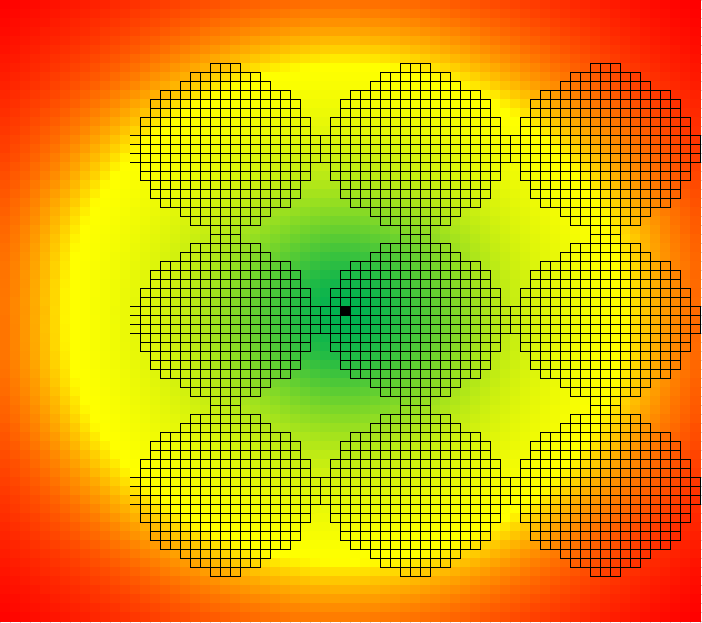
\includegraphics[width=0.9\textwidth]{pics/flux_map}
	\caption{Foil locations compared to the beam center.}
	\label{fig:flux_map}
\end{figure}   

The multiple-hole extraction system was also tested and the results were compared to simulations. Figure \ref{fig:chamfered} shows the non-optimized beam spot on the target. Note that the hot spots (darker) can be observed exactly where simulations show they would be, as shown in Figure \ref{fig:heat maps} (a). The irregular pattern is due to an attempt to remedy the situation by chamfering a few holes on the vacuum side to about $60^{\circ}$ in order to achieve an arrangement closer to a pierce-like angle geometry, and thus reducing the heat flux by spreading the individual beamlets. However, the chamfering also enlarged the holes, leading to increased current in the beamlets, counteracting the intended reduction.

\begin{figure}
	\centering
	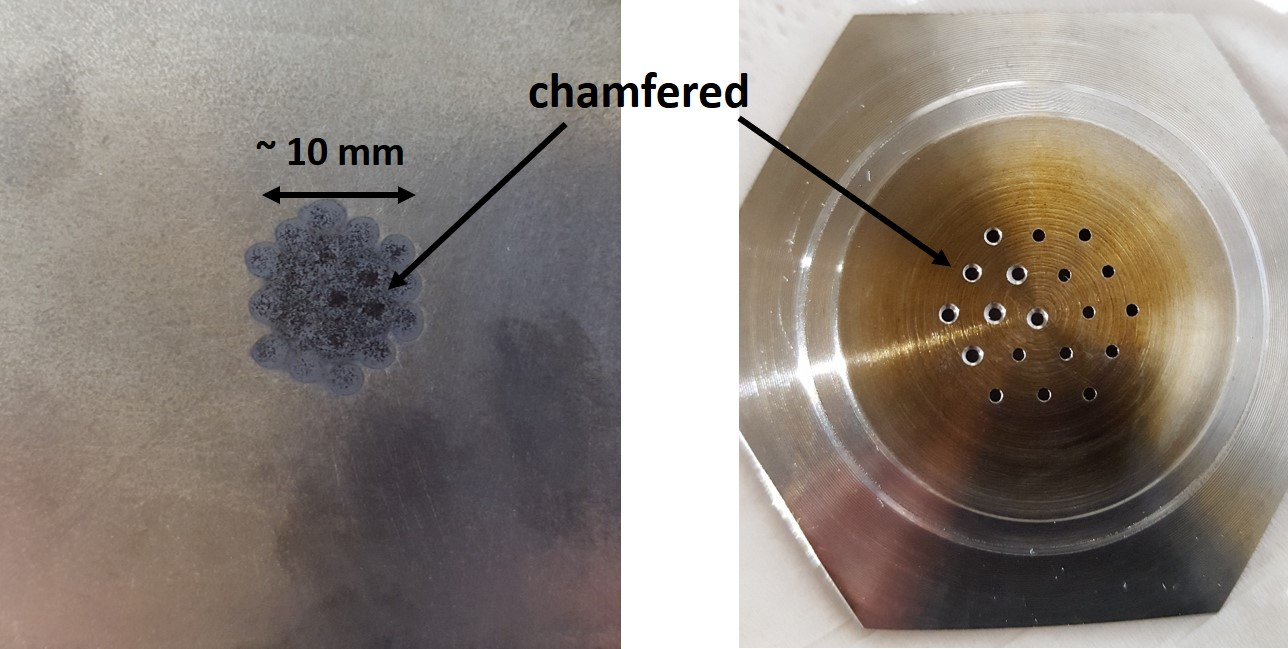
\includegraphics[width=0.9\textwidth]{pics/chamfered}
	\caption{Non-optimized design with a few chamfered holes and the corresponding beam spot.}
	\label{fig:chamfered}
\end{figure}  

Figure \ref{fig:optimized_notChamfered} shows the beam spot of the optimized extraction plate. Note that the beam size is accurately predicted by simulations, and it is similar in size as the non-optimized plate. The neutron flux at the central location was increased by a factor of 3.5 with such an arrangement. 

\begin{figure}
	\centering
	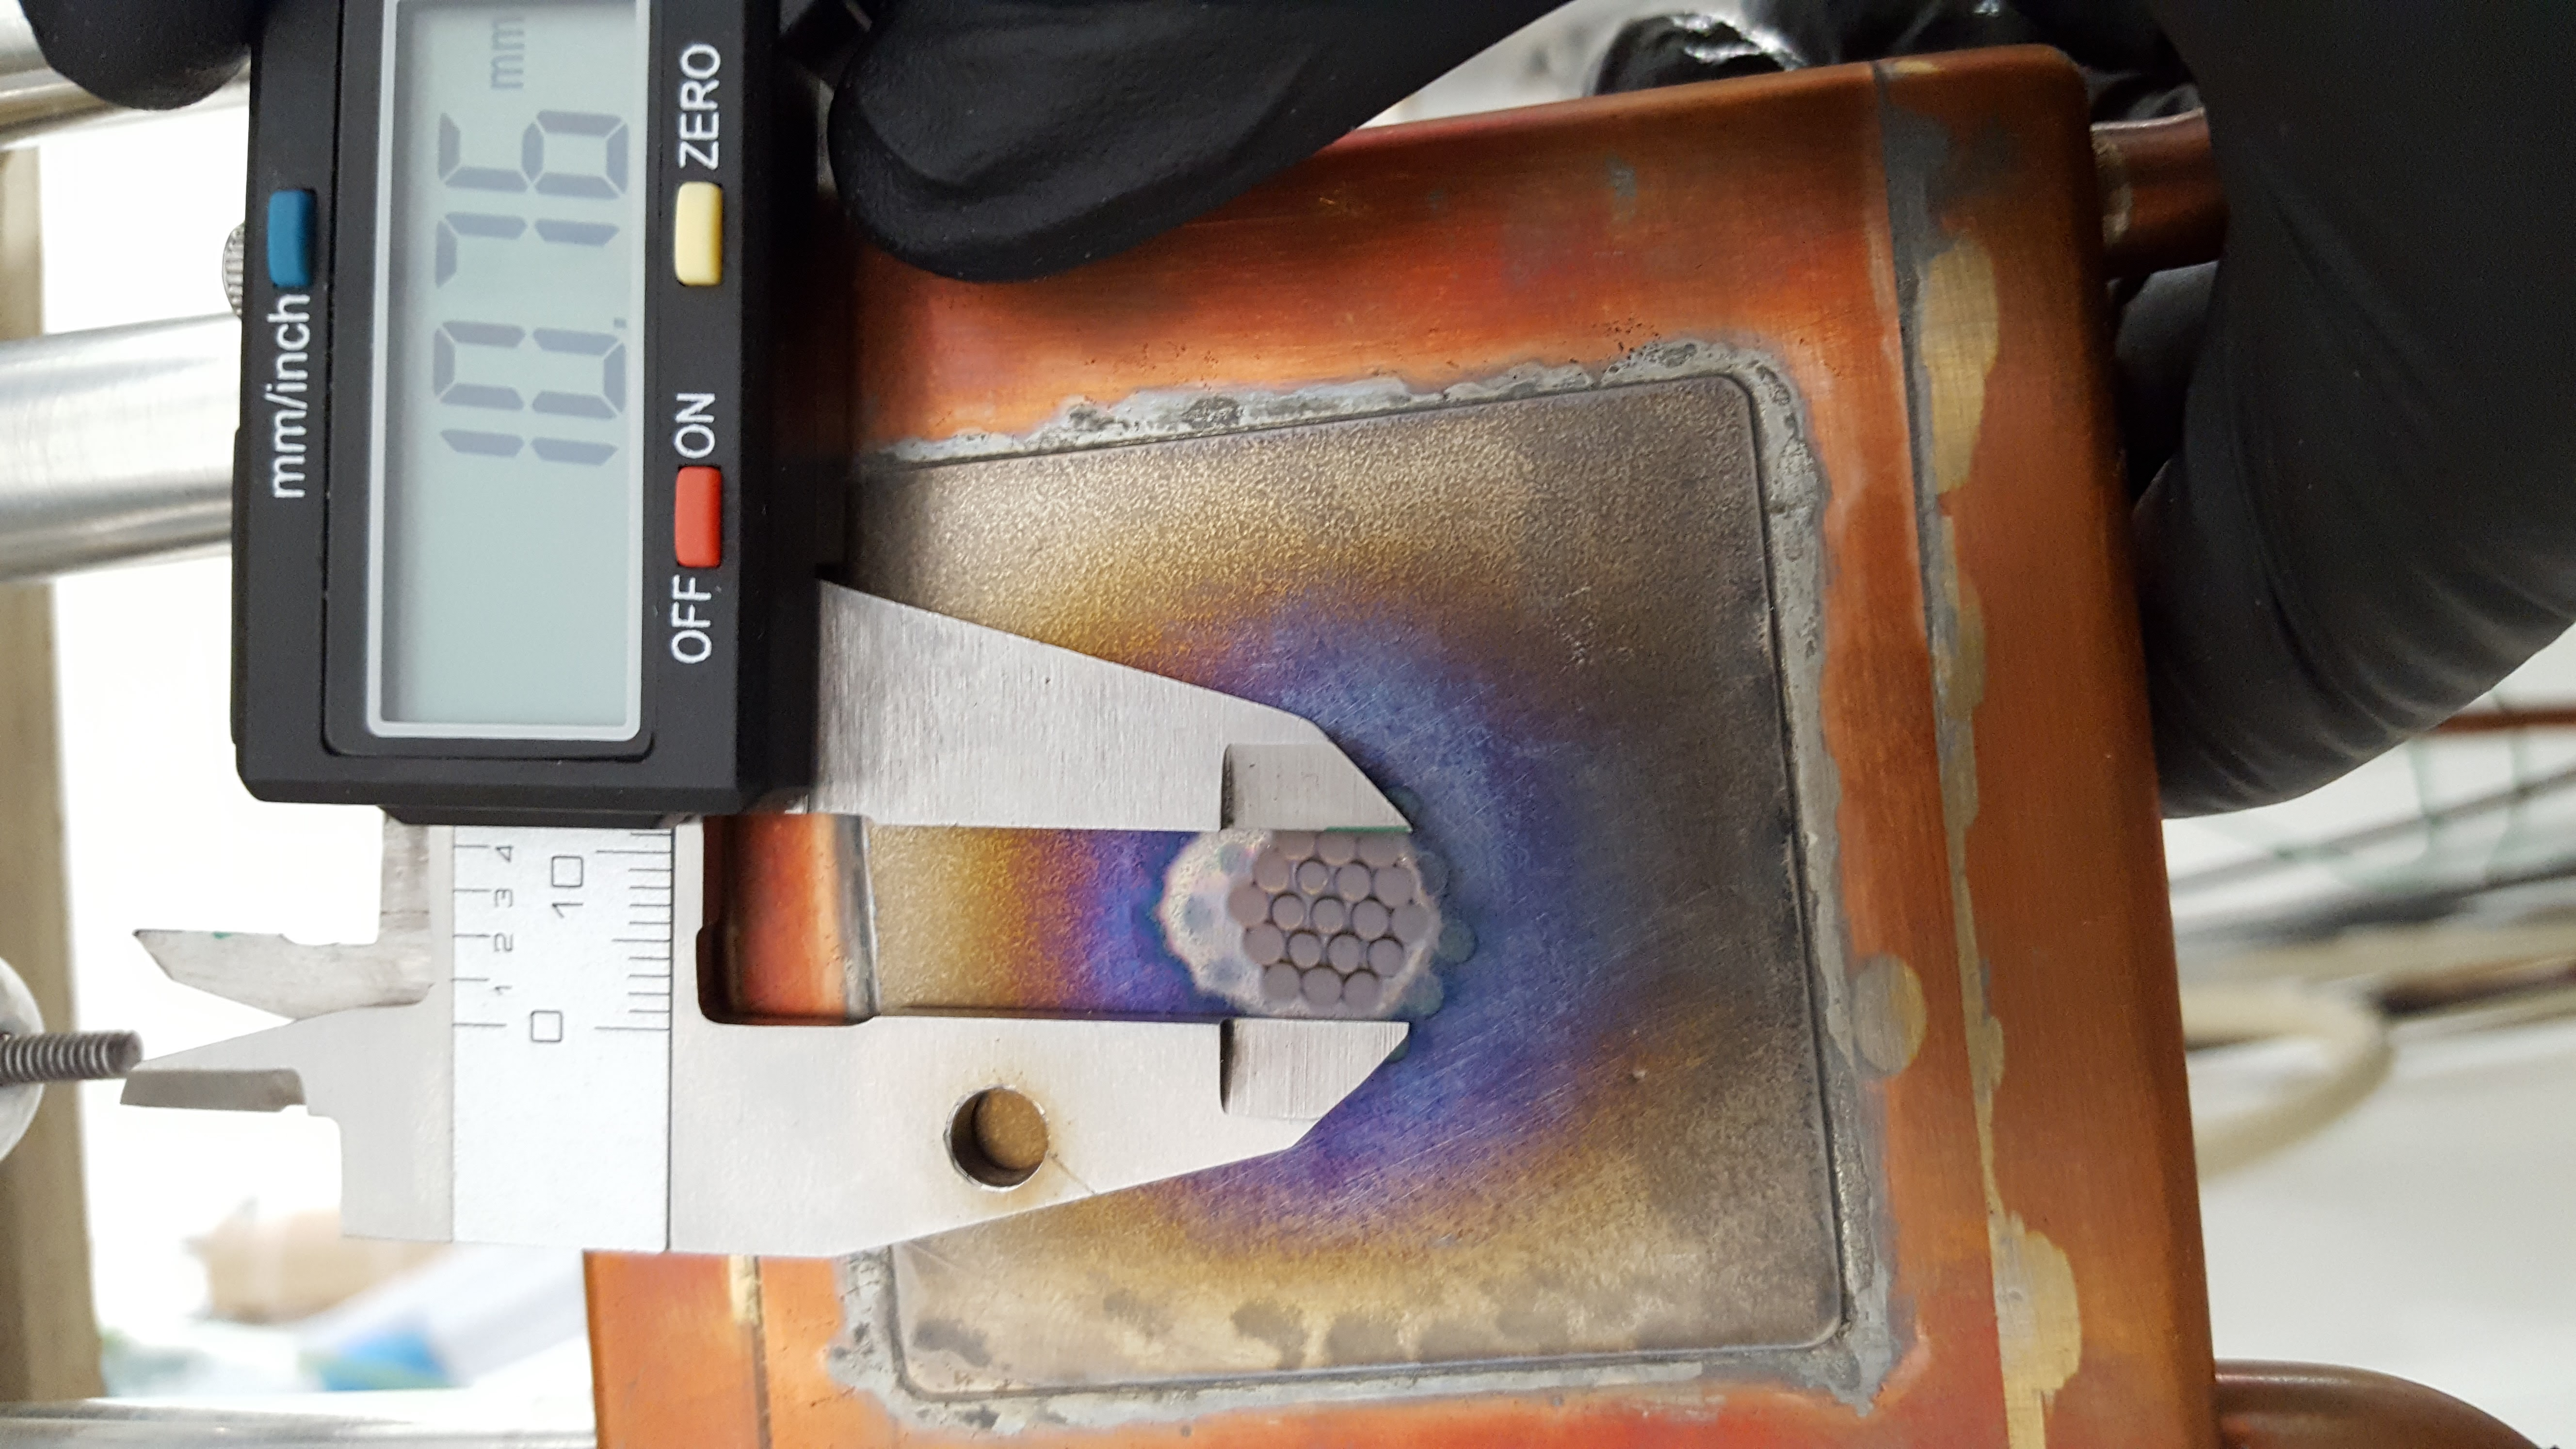
\includegraphics[width=0.9\textwidth]{pics/optimized_notChamfered}
	\caption{Optimized design and resulting beam spot.}
	\label{fig:optimized_notChamfered}
\end{figure}  

The variations in color due to the deuterium beam on the surface of the titanium are an indication of the amount of hydrogen absorbed. We noticed that after a few minutes of irradiation, the color was black while after a long time (hours) of irradiation, the color becomes light gray.  

\section{Conclusions and Outlook}

The HFNG is a multi-purpose versatile neutron generator that has been well characterized in terms of flux and energy distribution. Reliable simulation tools were developed coupled with experimental validation of the parameters of interest. Simulations included beam optics, heat transfer, neutron flux and energy distribution.

Moreover, neutron reflection studies are being investigated in order to increase the neutron fluence in the sample location. Heavy elements such as lead provide good reflection properties minimizing the energy loss per collision, which translates into an overall lower degradation of the energy spectrum. 

The heat removal capability of the target is one of the most important limiting parameters for neutron flux increase since hydrogen degases from titanium if high enough temperatures are achieved. Moreover, the neutron spot size must remain small for the flux to increase linearly with current. It is possible to increase the yield by spreading the beam spot, but that would not correspond to a linear increase in flux. 

\section{Acknowledgments}

We gratefully acknowledge a grant from the University of California Office of the President.
	
Work supported by NSF Grant No. EAR-0960138, U.S. DOE LBNL Contract No. DE- AC02-05CH11231, and U.S. DOE LLNL Contract No. DE-AC52-07NA27344.
	
\section*{References}
	
\bibliography{mybibfile}
	
\end{document}